\chapter{Background}
\label{chapter:Background}
This chapter provides the necessary theoretical an technological background topics of the thesis.

\section{Axioms of Linguistic Architectures}
\label{section:AxiomsOfLinguisticArchitectures}
This section summarizes axioms of linguistics architectures.
Axioms are outlined in \cite{DBLP:conf/sle/Lammel16} and refined in \cite{HeinzLV17}.
§\ref{subsection:Parthood} introduces the axiomatization for \gls{Parthood}
§\ref{subsection:Fragments} 

Axioms are presented in First Order Logic and formalization is taken from \cite{HeinzLV17}.
The universe to draw elements from is represented by the \Entity-predicate:
\begin{align*}
\forall x.\Entity(x).
\end{align*}
We assume it holds for everything of interest, hence such things are called \textit{entities}.

Linguistic architectures intend to describe software from language centric point of view, thus we provide specializations of entities for languages:
\begin{align*}
&\Set(x) \Rightarrow \Entity(x).\\
&\Language(x) \Rightarrow \Set(x).
\end{align*}
There are entities representing sets in a mathematical sense, and there are sets representing (formal-) languages in the sense of theoretical computer science.

On the other hand, we provide specializations for entities involved in software engineering terminology:
\begin{align*}
&\Artifact(x) \Rightarrow \Entity(x).\\
&\File(x) \Rightarrow \Artifact(x).\\
&\Folder(x) \Rightarrow \Artifact(x).
\end{align*}
There are entities representing all kinds of digital artifacts, e.g. files and folders.
Files represent persistent data resources, locatable either trough file systems or web services.
Folders represent locatable collections of files.
The intended use and semantic of these predicates is not meant to differ from intuitive, every day use.


\subsection{Parthood}
\label{subsection:Parthood}
\Gls{Parthood} is the essential relationship when reasoning about \gls{Correspondence} and \gls{Conformance} among artifacts within linguistic architectures \cite{DBLP:conf/sle/Lammel16} \cite{HeinzLV17}.
It describes the relation between entities and their constituent parts.
The study of \gls{Parthood} and its derivatives is \gls{Mereology} \cite{DBLP:journals/dke/Varzi96} \cite{SEP:Mereology}.
In the context of linguistic architectures we assume most entities to be
composed of several conceptual or physical parts.
In short, such entities are the sum of its parts.
That is, programs may compiled from many files, systems consists of several disjoint but dependent components, a \gls{Java} class is made up of methods and fields, etc.
Furthermore such entities are considered to be \textit{mereologically invariant}, i.e. if one part changes, the whole changes as well. 
Axiom \ref{axiom:PartOf} captures \gls{Parthood} at its most basic level.
\begin{axiom}[\partOf]
\label{axiom:PartOf}
\begin{align*}
&\partOf(p,w)
\Rightarrow
\Entity(p) \wedge \Entity(w).\\
&\partOf(p,w)
\Leftarrow
p \text{ is a constituent part of } w.
\end{align*}
\end{axiom}
\Gls{Parthood} is usually considered to be reflexive, antisymmetric and transitive \cite{DBLP:journals/dke/Varzi96} \cite{SEP:Mereology}, thus facilitating a partial order:
\begin{align*}
&\partOf(p,p). &\text{Reflxivity}\\
&\partOf(p,w) \wedge \partOf(w,p)
\Rightarrow
p = w. &\text{Antisymmertry}\\
&\partOf(p,w) \wedge \partOf(w,u)
\Rightarrow 
\partOf(p,u). &\text{Transitivity}
\end{align*}
The irreflexive \gls{Parthood} relationship is called proper:
\begin{align*}
&\properPartOf(p,w)
\Rightarrow
\Entity(p) \wedge \Entity(w).\\
&\properPartOf(x,y)
\Leftarrow
\partOf(x,y) \wedge \neg \partOf(y,x).
\end{align*}
Proper \gls{Parthood} is the strict order induced by normal \gls{Parthood}.
Figure \ref{figure:SchematicProperPart} shows a schematic illustration of proper parts.
\begin{figure}[h!]
\begin{center}
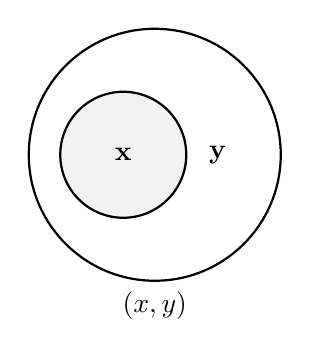
\begin{tikzpicture}[scale=0.8]
\draw[draw=black,thick](0,0)circle(2 and 2);
\draw[fill=gray!10,draw=black,thick](-0.5,0)circle(1 and 1);
\draw(-0.5,0)node{\textbf{x}};
\draw(1,0)node{\textbf{y}};
\node[anchor=north] at (current bounding box.south) {$\properPartOf(x,y)$};
\end{tikzpicture}
\end{center}
\caption{A schematic depiction of Proper Parthood}
\label{figure:SchematicProperPart}
\end{figure}
This Venn-style diagram depicts the scenario where $x$ is certainly a part of $y$, however $y$ is not a part of $x$.
In general proper \gls{Parthood} is a asymmetric relationship:
\begin{align*}
&\properPartOf(x,y) 
\Rightarrow
\neg \properPartOf(y,x).
&\text{Asymmetry}
\end{align*}

\Gls{Mereology} also allows for the notion of atomicity \cite{DBLP:journals/dke/Varzi96} \cite{SEP:Mereology}, i.e. atomic parts which cannot be decomposed in further parts:
\begin{align*}
\atomicPart(x)
\Leftarrow
\not \exists p.\properPartOf(p,x).
\end{align*}
Atomicity is later used to distinguish cases for \gls{Correspondence} and \gls{Conformance} (see §\ref{subsection:Correspondence} and §\ref{subsection:Conformance}).

\subsection{Fragments}
\label{subsection:Fragments}
\Glspl{Fragment} are a specialization of entities intended to capture the endogenous, mereological decomposition of artifacts \cite{HeinzLV17}.
Axiom \ref{axiom:Fragment} defines  \glspl{Fragment} as artifacts, which are neither files nor folders, and are properly embedded in at least one other artifact.
For instance, consider the syntactical decomposition of \gls{Java} classes, i.e. the class \gls{Fragment} contains method and field \glspl{Fragment}.
\begin{axiom}[\Fragment]
\label{axiom:Fragment}
\begin{align*}
&\Fragment(f) 
\Rightarrow
\Artifact(a) \wedge \neg(\File(f) \vee \Folder(f)).\\
&\Fragment(f) 
\Rightarrow 
\exists a.\Artifact(a) \wedge \properPartOf(f,a).
\end{align*}
\end{axiom}
We emphasize the proper \gls{Parthood} here, since not all authors necessarily consider \partOf~ to be reflexive \cite{DBLP:conf/sle/Lammel16} \cite{HeinzLV17}.
However, we previously distinguished between reflexive and irreflexive \gls{Parthood} and if we were to use reflexive \gls{Parthood} for the definition of the \Fragment-predicate it would be a tautology:
\begin{align*}
&\Fragment(f) 
\Rightarrow 
\exists a.\Artifact(a) \wedge \partOf(f,a).
&\text{Tautology}
\end{align*}
Since $\Fragment(f)$ implies $\Artifact(f)$ and \partOf~ is reflexive there is always an artifact for a \gls{Fragment} the latter is a part of, that is the \gls{Fragment} itself.

From the specification of \glspl{Fragment} we can first specialize the proper \gls{Parthood} predicate:
\begin{align*}
&\fragmentOf(f,x) 
\Rightarrow
\Fragment(f) \wedge \Artifact(x).\\
&\fragmentOf(f,x) 
\Leftarrow
\Fragment(f) \wedge \Artifact(x) \wedge \properPartOf(f,x).
\end{align*}
This is just a restriction of domain and range facilitating a special semantic.
Secondly, we can describe the process of fragmentation:
\begin{align*}
\partOf(p,w) \wedge \Fragment(w)
\Rightarrow
\Fragment(p).
\end{align*}
The \gls{Fragment} nature propagates top-down alongside the order of \gls{Parthood}, i.e. if an entity is a \gls{Fragment} all parts are also \glspl{Fragment} \cite{HeinzLV17}.

\subsection{Correspondence}
\label{subsection:Correspondence}
\Gls{Correspondence} is the relationship between to \glspl{Artifact} denoting both represent the same data in the sense that they are mereologically similar \cite{HeinzLV17}.
It usually occurs as exogenous relationship, i.e. the involved \glspl{Artifact} do not belong to the same \gls{Language}, for instance \gls{XML} and \gls{JSON} may contain the same information.

In order to axiomatize \gls{Correspondence} properly we need to introduce two other relationships first:
\begin{description}[align=left]
\item[\represents]
The relationship denoting that an \gls{Artifact} is a \gls{Representation} or \gls{Manifestation} of an entity.
\begin{align*}
&\represents(a,e)
\Rightarrow
\Artifact(a) \wedge \Entity(e).\\
&\represents(a,e)
\Leftarrow
a \text{ is a representation of } e.
\end{align*}

\item[\sameAs]
The relationship denoting two artifacts represent the same entity.
\begin{align*}
&\sameAs(x,y)
\Rightarrow
\Artifact(x) \wedge \Artifact(y).\\
&\sameAs(x,y)
\Leftarrow
\exists e.\represents(x,e) \wedge \represents(y,e).
\end{align*}
\end{description}

The axiomatization of \gls{Correspondence} from \cite{HeinzLV17} is slightly altered with emphasis of irreflexive proper \gls{Parthood}, Otherwise it would not work with axiom \ref{axiom:PartOf}.
\begin{axiom}[\correspondsTo]
\label{axiom:CorrespondsTo}
~\newline
\resizebox{\linewidth}{!}{
\begin{minipage}{\linewidth}
\begin{align*}
\correspondsTo(x,y)
&\Rightarrow
\Artifact(x) \wedge \Artifact(y).\\
\correspondsTo(x,y)
&\Leftarrow
(\forall px.\properPartOf(px,x) \Rightarrow \exists py.\properPartOf(py,y) \wedge \correspondsTo(px,py))\\
&\wedge
(\forall py.\properPartOf(py,y) \Rightarrow \exists px.\properPartOf(px,x) \wedge \correspondsTo(py,px))\\
&\vee
(\not\exists p.\properPartOf(p,x) \vee \properPartOf(p,y)) \wedge \sameAs(x,y).
\end{align*}
\end{minipage}
}
\end{axiom}
Axiom \ref{axiom:CorrespondsTo} defines \gls{Correspondence} recursively:
\begin{enumerate}[align=left,label=\textbf{Case \Roman*},ref={\Roman*}]
\item
If both \glspl{Artifact} is atomic in the sense it cannot be decomposed in further parts, we check whether both artifacts represent the same data.

\item
Else, if at least one \gls{Artifact} is not atomic, then for each proper part of one \gls{Artifact} has to be a corresponding part in the other and vice versa.
\end{enumerate}
This axiomatization demands a strict one-to-one correspondence in its recursive clause which occurs in reflexive cases, i.e. $\correspondsTo(x,x)$, but may be to strict for real-world applications \cite{DBLP:conf/sle/Lammel16}.

\subsection{Conformance}
\label{subsection:Conformance}
\Gls{Conformance} is the relationship between two \glspl{Artifact} denoting one satisfies the syntax specification given by the other \cite{HeinzLV17}.
This satisfaction is also meant to mereologically decomposable, i.e. there are parts of one \gls{Artifact} specified by a part of the other.


In order to axiomatize \gls{Conformance} properly we need to introduce two other relationships first:
\begin{description}[align=left]
\item[\defines]
The relationship simply denoting an \gls{Artifact} contains the definition of an entity.
\begin{align*}
\defines(a,e)
&\Rightarrow
\Artifact(a) \wedge \Entity(e).\\
\defines(a,e)
&\Leftarrow
a \text{ is a definition for } e.
\end{align*}

\item[\elementOf]
The relationship denoting set-theoretic membership.\footnote{We do not use the \elementOf axiom for \glspl{Artifact} and \glspl{Language} from \cite{HeinzLV17}, because it introduces the possibility for infinite mutual recursion:
\begin{align*}
\elementOf(a,l)
&\Rightarrow
\Artifact(a) \wedge \Language(l).\\
\elementOf(a,l)
&\Leftarrow
\exists s.\defines(s,l) \wedge \conformsTo(a,s)
\end{align*}}
\begin{align*}
\elementOf(e,s)
&\Rightarrow
\Entity(e) \wedge \Set(s).\\
\elementOf(e,s)
&\Leftarrow
e \in s.
\end{align*}


\end{description}


The axiomatization of \gls{Conformance} from \cite{HeinzLV17} is also slightly altered with emphasis of irreflexive proper \gls{Parthood}, Otherwise it would not work with axiom \ref{axiom:PartOf}.
\begin{axiom}[\conformsTo]
\label{axiom:ConformsTo}
~\newline
\resizebox{\linewidth}{!}{
\begin{minipage}{\linewidth}
\begin{align*}
\conformsTo(a,d)
&\Rightarrow
\Artifact(a) \wedge \Artifact(d).\\
\conformsTo(a,d)
&\Leftarrow
(\forall pa.\properPartOf(pa,a) \wedge \exists pd.\properPartOf(pd,d) \wedge \conformsTo(pa,pd))\\
&\vee \exists l.\defines(d,l) \wedge \elementOf(a,l).
\end{align*}
\end{minipage}
}
\end{axiom}
Axiom \ref{axiom:ConformsTo} defines \gls{Conformance} recursively:
\begin{enumerate}[align=left,label=\textbf{Case \Roman*},ref={\Roman*}]
\item
If both \glspl{Artifact} is atomic in the sense it cannot be decomposed in further parts, we check whether one \gls{Artifact} defines a language the other \gls{Artifact} is an element of.

\item
Else, if at least one \gls{Artifact} is not atomic, then for each proper part of one \gls{Artifact} has to be a proper part in the other \gls{Artifact} it conforms to.
\end{enumerate}


\section{Traceability}
\label{section:Traceability}
This section provides brief background on the topic of \gls{Traceability}, i.e. its objectives and terminology.
\Gls{Traceability} as a desired property of software systems and their development process originates from requirement engineering, i.e.
how do we validate or verify that all requirements are met \cite{Winkler:2010:STR:1861285.1861287}?
Or more precisely: on what data can we base such validation or verification?
An answer to these questions is motivated by observations on development processes of software systems.
Because such a process usually has an iterative and incremental nature, we can reasonably assume engineering activities to leave \glspl{Trace} which reflect the performed action.

Modern day \gls{Traceability} objectives are not limited to requirement validation.
It is also regarded as a desirable property supporting engineering activities, e.g. change impact analysis or dependency analysis \cite{DBLP:books/daglib/p/GotelCHZEGDAMM12} \cite{Gotel94ananalysis}.
This feeds to the overall topic of program comprehension.

\begin{definition}[Trace]
content...
\end{definition}

\begin{definition}[Trace Link]
content...
\end{definition}


\begin{definition}[Traceability Recovery]
content...
\end{definition}


\section{Technical Background}


\subsection{\megalxtext}
\cite{DBLP:conf/sattose/BaggeZ14}
\cite{DBLP:journals/entcs/FavreN05}

\cite{DBLP:conf/ecmdafa/LammelV14}
\cite{DBLP:conf/models/FavreLV12}
\cite{DBLP:conf/sle/Lammel16}

\cite{LukasHaertelBScThesis}

\subsection{Java Architecture for XML Binding (JAXB)}

\subsection{Hibernate}

\subsection{Another Tool For Language Recognition (ANTLR)}
\cite{Parr:2013:DAR:2501720}

